% !TeX root = ./main.tex

\documentclass[fontsize=12pt]{scrartcl}
\usepackage[english]{babel}
\usepackage[utf8]{inputenc}
\usepackage{csquotes}
\usepackage[
	backend=biber,
	style=numeric,
	sorting=ynt
]{biblatex}
\usepackage{graphicx}
\graphicspath{{images/}}
\usepackage[table,x11names,dvipsnames,table]{xcolor}
\addbibresource{references.bib}
\PassOptionsToPackage{hyphens}{url}
\usepackage[
    colorlinks,
    linkcolor={red!50!black},
    citecolor={blue!50!black},
	urlcolor={blue!80!black}]{hyperref}
\usepackage{amssymb}
\usepackage{amsmath}
\usepackage{multirow}
\usepackage[automark,headsepline]{scrlayer-scrpage}
\usepackage{vmargin}
\usepackage{hyphenat}
\usepackage{subcaption}
\usepackage[section]{placeins}
\usepackage{pdfpages}
\usepackage[inline]{enumitem}
\usepackage[font=small]{caption}
\usepackage{wrapfig}
% \usepackage[toc,page]{appendix}
\usepackage[smartEllipses]{markdown}
\usepackage{chngcntr}
\counterwithin{figure}{section}
\counterwithin{table}{section}

\definecolor{light-gray}{gray}{0.9} 
% \setmarginsrb{3.5 cm}{1.5 cm}{2.5 cm}{2 cm}{1 cm}{1.5 cm}{1 cm}{1.5 cm}
\setlength{\parskip}{10pt plus 1pt minus 1pt}
\linespread{1.3}

\title{Analysis of Courses of Study to Predict Consequences of Educational Choices Using Machine Learning}
\author{Moritz Nipshagen}
\date{\today}											% Date

\makeatletter
\let\thetitle\@title
\newcommand\theauthor{M. Nipshagen}
\let\thedate\@date	
\makeatother

\clearpairofpagestyles
\cfoot[\pagemark]{\pagemark}
% \lehead{\headmark}
\lohead{\nohyphens{\parbox{0.6\textwidth}{\small{\thetitle}}}}
% \rohead{\headmark}
\rohead{\small{\theauthor}}
\pagestyle{scrheadings}

% \pagestyle{fancy}
% \fancyhf{}
% \rhead{\small{\theauthor}}
% \lhead{\small{\thetitle}}
% \cfoot{\thepage}

\newcommand{\mycaption}[2]{\caption[#1]{#1\\#2}}

\begin{document}

%%%%%%%%%%%%%%%%%%%%%%%%%%%%%%%%%%%%%%%%%%%%%%%%%%%%%%%%%%%%%%%%%%%%%%%%%%%%%%%%%%%%%%%%%
\pagenumbering{gobble}
\begin{titlepage}
	{
		\centering
		\vspace*{0.5 cm}
		\includegraphics[scale = 0.25]{wappen.png}\\[1.0 cm]	% University Logo
		\textsc{\LARGE Osnabrück University}\\
		{\Large School of Human Sciences\\
		Institute of Cognitive Science}\\[1.0 cm]	% University Name
		{\large Bachelor Thesis\\
		In Partial Fulfilment of Requirements\\
		For the Degree of Bachelor of Science}\\[0.5 cm]				% Course Name
		% \textsc{\Large Course Code: 8.3304}\\[0.5 cm]				% Course Code
		\rule{\linewidth}{0.2 mm} \\[0.4 cm]
		{ \LARGE \bfseries \thetitle }\\
		\rule{\linewidth}{0.2 mm} \\[0.75 cm]
		{\large 
			Moritz Nipshagen\\
			April, 2019\\
		}
	}
	\vfill
	{\noindent
		% Moritz  Nipshagen\\
		B.Sc. Cognitive Science, 7th Semester\\
		963496\\
		\href{mailto:mnipshagen@uos.de}{mnipshagen@uni-osnabrueck.de}\\
		Schlosswall 17\\
		49074 Osnabrück
	}
	\par
	{\noindent
		1st Supervisor: Dr. Tobias Thelen\\
		2nd Supervisor: Prof. Dr.-phil. Kai-Uwe Kühnberger
	}
	
	
	% {\large \thedate}\\[2 cm]
	
\end{titlepage}
\pagebreak
\vspace*{\fill}
{
	\hfil \Large\textit{Page intentionally left blank} \hfil
}
\vspace*{\fill}

%%%%%%%%%%%%%%%%%%%%%%%%%%%%%%%%%%%%%%%%%%%%%%%%%%%%%%%%%%%%%%%%%%%%%%%%%%%%%%%%%%%%%%%%%

% !TeX root = ./main.tex

\section*{Abstract}
Students drop out of their program for different reasons. They might have noticed that their current program is not a good fit and look for a better alternative, or they might have had an opportunity for something they considered more valuable than finishing their degree. More problematic are students that drop out due to being overwhelmed, not fulfilling expectations or struggling with extracurricular burdens. Since dropping out of a program often incurs a high financial as well as social cost, it is important to provide personalized interventional support to those students. Using data mining techniques, the large amounts of data collected by universities and institutions can be analyzed. However, most work done in this field has been done on small datasets; additionally some have used only one specific algorithm to deduce a result. The "Leibniz-Institut für Bildungsverläufe" (LIfBi) supplies the expansive "National Education Panel Study" (NEPS) dataset, a longitudinal study with an encompassing breadth of variables recorded. This thesis shows the process of working with the NEPS dataset to create a dataset fit to be used with machine learning. It further employs and compares several machine learning models, whose weights are then analyzed to work out important features for study success.
\pagebreak

\tableofcontents
\listoftables
\listoffigures
\pagebreak

\pagenumbering{arabic}
\setcounter{page}{1}
%%%%%%%%%%%%%%%%%%%%%%%%%%%%%%%%%%%%%%%%%%%%%%%%%%%%%%%%%%%%%%%%%%%%%%%%%%%%%%%%%%%%%%%%%

% !TeX root = ./main.tex

\section{Introduction}
Accurately supporting students and preventing dropouts is one of the more daunting tasks universities face in the current age. Students have different reasons for dropping out of their program, and not all of them are preventable nor should they be prevented. If a student finds a better fit elsewhere or has a grant opportunity to follow they should not be held back. However, those that drop out because they struggle with the subjects or extracurricular burdens, should be actively supported. For a personalized intervention to be effectively planned and executed, struggling students need to be identified early on. In order to identify students that struggle to complete their program, those features must be identified which constitute to a successful study episode.\\
Universities and institutions collect a wide range of data on students' background, progress and success. To analyze these large amounts of data, techniques from fields like data mining, artificial intelligence and machine learning are useful. Bringing data mining techniques into the educational setting has been a growing scientific field\cite{Romero.2013}. There has been work on high school students to predict and support their study success \cite{Kaplan.1997, Tamhane.2014, Lakkaraju.2015} and faculty specific research \cite{Kovacic.2012, Nikolovski.April2015}. Most of this work is done on small datasets (< 20 variables), or employ only simple techniques for prediction, like logistic regression. Some papers employed decision trees to evaluate and explain the students' success rate. Only one paper was found that used machine learning in a longitudinal study \cite{Tamhane.2014}. The data used in those papers was created for the study itself and did not seem to be publicly available.\\
After features are identified, there is the important and difficult task to support students in achieving their goals. There is ongoing research on this matter. One of those projects is the SIDDATA project \cite{Osada.2019}. SIDDATA aims to provide a data-driven assistant to help students formulate, work towards and achieve individual goals. One main aspect of this assistant is to integrate previously unconnected data sources and provide a combined overview. This can include but is not limited to data from campus management systems, open educational resources and workshop and courses offered at universities.

To identify relevant features, there needs to be representative data to analyze and derive the features from. The mentioned papers all were not located in western or central Europe and their dataset were not publicly available. Hence, there was no reference dataset directly available which is representative for the students in Germany. Websites like \href{https://www.re3data.org/}{re3data.org}, \href{https://nces.ed.gov/datalab/index.aspx}{nces.ed.gov/datalab} and \href{http://educationaldatamining.org/}{educationaldatamining.org} supply a limited selection of datasets concerning education. All of these did not satisfy the crieteria of being longitudinal, large scale and representative. However, the "Leibniz-Institut für Bildungsverläufe" (LIfBi) provides the "National Education Panel Study" (NEPS) dataset\cite{Weinert.}. It features several cohorts (from newborns over kindergarten and school to first-year students and young adults), each a longitudinal study following the participants over the span of several years. The quantitative and qualitative data compiled is exhaustive and with several thousand participants, it was the largest dataset to be found.\\

In line with the approach of the SIDDATA project, this thesis aims to provide a data-driven approach to identify relevant features for student success. This work outlines the process of surveying and preprocessing the NEPS dataset and provides insight into the structure and flaws of the convoluted dataset. Several machine learning algorithms are applied to the preprocessed data and the results analyzed and compared. When working with machine learning, it is important to keep in mind what one is predicting from which source and what this implies. This thesis is looking to predict the successful completion of a degree program. This is predicted from collected background information and episodical contextual information during the study episode. There is no information on skills gained, the quality of the study or the fit of the student for the program entailed. There is a plethora of positive reasons to not finish a study program, but this cannot be evaluated as there is no information on a student's reasoning for dropping out; if it was, it has been redacted. Finally, the important features of those algorithms are read out and discussed. The discussion also contains a more general part on the ethics of employing data mining and AI in education.

All code used for in this thesis can be found on the attached medium, the readme is attached in the appendix \ref{apx:readme}, or on \url{https://github.com/mnipshagen/thesis/}.

% !TeX root = ./main.tex

\section{The Dataset}
\label{sec:data}
This thesis analyzes data from the National Educational Panel Study: Starting Cohort First-Year Students (\cite{Weinert.}). From 2008 to 2013, NEPS data was collected as part of the Framework Program for the Promotion of Empirical Educational Research funded by the German Federal Ministry of Education and Research (BMBF). As of 2014, NEPS is carried out by the Leibniz Institute for Educational Trajectories (LIfBi) at the University of Bamberg in cooperation with a nationwide network.
\\
The main reason to use the NEPS dataset was its longitudinal setup, the large number of participants and the variety of the questions. The dataset is is unique in its size, breadth and completeness among comparable records. Other resources in this area are often course specific, e.g. considering the progress students made over the roughly half a year in a single subject. Some were considering online courses on sites like "Udacity"\footnote{\url{www.udacity.com}}, which do not generalize well for higher education. Although, they are a lot easier to record information from since all interaction with the students is digital. Resources similar to the NEPS dataset were considerably smaller. Hence, the encompassing nature of the dataset seemed most fitting for the task of predicting drop outs. The main downside for this work using NEPS is that the dataset has little quantitative information on the progress of the study; there is no information on ECTS per semester or grade per course, nor extensive information on courses done.
\\
The NEPS database features several cohorts. The dataset chosen for this work, was the 5th cohort (SC5) "First-Year Students" in its most current version 11. This cohort data was collected from 2010 to 2016, by conducting two interviews each year on the current state of the life of the students. This involved quantitative factors of their academic career so far and their socio-economic situation, as well as qualitative factors like how they feel about their career chances or how happy they are. The data is structured in two different time formats. Firstly, there is panel data, which holds data from a certain point in time. Since it was a longitudinal study, several panel points in time were aggregated into one group, meaning each interview can be uniquely identified by the student's ID (variable \textit{ID\_t}) and the wave number. Secondly, there is episodic data, which is called "spell data". A spell is one episode of the context saved in that specific file. For example, a spell in the spSchool file identifies one school episode (e.g. until switching schools or achieving a certificate) or a spell in the spEmp file represents one episode of employment from start until termination. Spells have no fixed length, but rather are defined their start and end date depending on the context they are collected in, e.g. the school group would have one spell for each school visited or diploma achieved; switching schools or achieving an intermediate diploma would constitute a new spell. Spells could either be completed or ongoing. If a spell is ongoing for several interviews, there will be several rows for this spell and once it is done, a new integrated row for the completed spell will be created. 
The collected data was grouped and structured into different files (for an overview see figure \ref{fig:file_overview}). The LIfBi also provided some aggregated data files. Most of the variables observed are either ordinal or nominal with few real valued variables. % add something
Depending on the access level, there are less anonymized or redacted variables available. This work uses the offsite, downloadable version and as such have no access to free text answers as well as having some information redacted which might have made it easier to identify a single student, e.g. the exact study program, institution or state of study.
\begin{figure}[ht]
    \centering
    \includegraphics[width=.75\textwidth]{file_overview}
    \mycaption{Overview of used NEPS files}{An overview of all files in the NEPS dataset. Those marked in gray have not been used in the analysis.}
    \label{fig:file_overview}
\end{figure}
% \begin{description}
% 	\item [Computer Assisted Telephone Interview] CATI
% 	\item [Computer Assisted Web Interview] CAWI
% 	\item [Child] Children stuff
% 	\item [Child Cohabilitation] Living with children
% 	\item [Courses] Courses done
% 	\item [Employment] Phases of Employment
% 	\item [Further Education] Additional Education
% 	\item [Gap] Gap years done
% 	\item [Internship] Internships done
% 	\item [Military] Military and Civil Service episode
% 	\item [Parental Leave] Taken Parental Leave
% 	\item [Partner] Special Someone Information
% 	\item [School] School Education
% 	\item [School External Exams] External Examinations
% 	\item [Sibling] Siblings
% 	\item [Unemployment] Non-Employment
% 	\item [Vocational External Exam] External Exams linked to Vocational Training
% 	\item [Vocational Preperation] Ehm?
% 	\item [Vocational Training] Vocational Trainings like Higher Education and Apprenticeships
% \end{description}

% !TeX root = ./main.tex

\section{Methodology}
By far the largest part of this work was the surveying and preprocessing of the data to transform it into a conforming format. "Conforming" means here that the result is usable by the different frameworks used for training. For this the the data files needed to be altered in such a way that per student only one row remained. These rows then can be appended to each study spell of the student, forming a coherent dataframe where each row represents one input vector plus the target value. The data is fed as an input vector, and several rows, containing information on the same variable is not simply convertible into one single vector, since one variable can only contain one value. The most simple appraoch would be to append all rows together, but since there are different amount of rows per student, all others would need to be padded to the maximum length, resulting in a larger amount of additional NaN values. Hence, another appraoch needed to be taken to aggregate the several rows. The preprocessed data could then be fed into the different machine learning algorithms used. The algorithms can be tuned with different hyperparameters slightly changing their behaviour. They learn the most important features to predict the outcome. For some of the models the learning can then be evaluated.\\
The data processing was handled with pandas (v0.24.2)\cite{WesMcKinney.2010} and numpy (v1.16.2)\cite{vanderWalt.2011}. The training and evaluation was done in scikit-learn (v0.20.3)\cite{Pedregosa.2011} and TensorFlow (v.1.13.1)\cite{Abadi.20160531}. The visualizations were created with matplotlib (v3.0.3)\cite{Hunter.2007} and seaborn (v.0.9.0)\cite{Waskom.2018}.

\subsection{Machine Learning}
In trying to remove human bias from the choice of important predicators, the predictions were made using machine learning algorithms. While a human observer might have a good intuition on what features impact study success more heavily, any human will be biased. According to merriam-webster\footnote{\url{https://www.merriam-webster.com/}, visited 30.04.2019} Machine Learning is "the process by which a computer is able to improve its own performance (as in analyzing image files) by continuously incorporating new data into an existing statistical model". The goal is that the algorithms extract knowledge from the supplied data, in order to make predictions in the future about similar data samples. There are different learning methods for machine learning. All models used and discussed here are supervised learning models.\\
While all models also are usable for regression tasks, the explanations here will focus on their application for classification. The introduction given here aims mostly at gaining an intuition and overview on those topics. For the mathematical formulation and in depth explanations refer to the work cited.

\subsubsection{Supervised Learning}
The task at hand is handled as a supervised learning task. That is, we have a set of data tuples, consisting of input vectors and their corresponding labels. The data is then split into two parts: one for training and one for testing the performance. Usually around 20\% of the data is kept apart for testing later. During training the model is then given the input vector to predict labels. The predicted labels are then compared with the known correct labels. This gives a score to evaluate the model and depending on which labels were wrong, the weights of the model are adjusted to achieve a better performance. This is repeated for all the samples of the training set, sometimes several times in so called epochs. After training is done, the model is shown the test input vectors and the predictions are compared to the test labels. However, this time the weights are not updated anymore. The resulting score is then a measure of how well the model generalized and performs on unseen data.

\subsubsection{Support Vector Machines}
\FloatBarrier
Support Vector Machines (SVM, also called Support Vector Networks) have been originally introduced in 1964 \cite{Aizerman.1964}. They were since then improved and exist in their current form since the 90s \cite{Boser.1992, Cortes.1995}. The underlying idea is to transform input vectors that are not linearly seperable into higher dimensional space. This transformation is expressed by the transformation function $\phi$, which is defined as $\phi: \mathbb{R}^n \rightarrow \mathbb{R}^m, m>n$. In this higher dimensional space the data then can be separated by a hyperplane (visualized in figure \ref{fig:svm_nonlineardata_whole}). The constructed hyperplane aims to maximize the distance to the data points of each class, to increase generalization and label new data with higher accuracy. The closest data points to the separation hyperplane are called the support vectors. After the construction of the hyperplane, the data and separator are mapped back to the original dimensionality, creating a non-linear separator from the linear separation plane.\\
\begin{figure}[ht] % linear and non-linear separable data
    \centering
    \begin{subfigure}{.5\textwidth}
        \centering
        \includegraphics[width=.8\textwidth]{svm_linear_scatter.png}
        \mycaption{Linearly Seperable Data}{An artificially created dataset that is easily linearly separable}
        \label{fig:svm_lineardata}
    \end{subfigure}%
    \begin{subfigure}{.5\textwidth}
        \centering
        \includegraphics[width=.8\textwidth]{svm_circle_scatter.png}
        \mycaption{Non-Linearly Separable Data}{The circular data structure makes it linearly inseparable. A non linear classifier would be needed.}
        \label{fig:svm_nonlineardata}
    \end{subfigure}
    \mycaption{Example Datasets}{Artificial example datasets to illustrate the difference between linearly and non-linearly separable data.}
\end{figure}
The projection into higher space and then back again, can be expressed as the inner (dot) product of the transformation of two vectors ($\langle\phi(x_n),\phi(x_n')\rangle$) and according to Mercer's Theorem this mapping can be done independently from the explicit transformation \cite{Jordan.2004}. This computation of the inner product of the transformation of two input vectors is called a kernel. Thus a kernel $K(x,x') = \langle\phi(x_n),\phi(x_n')\rangle$ maps $K: \mathbb{R}^n\times\mathbb{R}^n\rightarrow\mathbb{R}$ the dot product of two n-dimensional vectors to a real valued scalar. Avoiding to explicitly state the transform function in this way is called the "Kernel Trick"\cite{Theodoridis.2008}. There are several kernel functions that fulfill those properties and are widely used. Most simple is the linear kernel, which is also what the examples here illustrate. In training, several kernels were tested on the dataset:
\[
\begin{array}{ll}
    \text{linear} & (\langle x,x'\rangle)\\\nonumber
    \text{sigmoidian / hyperbolic tangent} & (\tanh{(\gamma\langle x,x'\rangle+r)})\\\nonumber
    \text{polynomial} & ((\gamma\langle x,x'\rangle+r)^d)\\\nonumber
    \text{gaussian radial basis function (rbf)} & (\exp{(-\gamma\lVert x,x'\rVert^2)})\\\nonumber
\end{array}
\]
While harder to solve, non-linear kernels do perform better on smaller feature spaces than a linear kernel.
\begin{figure}[ht] % composite of 3d transform
    \centering
    \begin{subfigure}{.33\textwidth}
        \centering
        \includegraphics[width=.8\linewidth]{svm_circle_3d.png}
        \caption{}
        % \caption{The circular dataset from \ref{fig:svm_nonlineardata} projected to 3-dimensional space using $T(x,y) \rightarrow (x, y, x^2+y^2)$. The data is now linearly seperable.}
        \label{fig:svm_nonlineardata_3dprojection} 
    \end{subfigure}%
    \begin{subfigure}{.33\textwidth}
        \centering
        \includegraphics[width=.8\linewidth]{svm_circle_3d_hyperplane.png}
        \caption{}
        % \caption{Projected dataset with separation hyperplane.}
        \label{fig:svm_nonlineardata_3dprojection_hyperplane}
    \end{subfigure}%
    \begin{subfigure}{.33\textwidth}
        \centering
        \includegraphics[width=.8\linewidth]{svm_circle_scatter_hyperplane.png}
        \caption{}
        % \caption{Data projected back into 2-dimensional space, including hyperplane projection. The linear hyperplane becomes a non-linear separation in lower dimensional space.}
        \label{fig:svm_nonlineardata_hyperplane}
    \end{subfigure} 
    \mycaption{SVM Projection Into a Higher Space}{(a) shows a possible transformation of the dataset from \ref{fig:svm_nonlineardata} to 3d space using $T(x,y) \rightarrow (x, y, x^2+y^2)$. (b) then shows a separating hyperplane that could be constructed by a SVM. (c) is the representation in 2d back from the transformed data and constructed hyperplane. The linear hyperplane now appears as a non-linear separator.
    Inspired by and derived from \cite{Kim.2013}.}
    \label{fig:svm_nonlineardata_whole}
\end{figure}

There are extensions to SVMs that allow for multiclass classification, which will not be further discussed here as they have no tangent with this work. The input vectors to SVMs must be real valued. To this day, SVMs are a benchmark for ML applications.
\FloatBarrier

\subsubsection{Decision Trees}
\FloatBarrier
Decision Trees are also known from outside computer science. The concept for decision making is the same as it is on a flowchart and as it is seen and used in offices for decision making and project management. The computer science tree and paper flowcharts function the same way. They consist of nodes and branches connecting them. The start node is called the root and if a node is terminal -- it does not branch further, it is called a leaf. Each node represents a feature, the branches from a node are the corresponding feature values and the leaves are target values. When classifying a sample, one starts at the root and then uses the feature value of the current feature node to decide which branch to follow until one reaches a leaf node. The leaf then determines the classification outcome. Decision Trees have intelligible feature weights, meaning that one can read out which features are closer to the root. The closer a feature is to the root, the higher is the importance of the information they are carrying for classification. See figure \ref{fig:dtc} for a simple example of a decision tree. Here the target variable is a binary decision of whether to go play tennis. There are three features: Outlook, wind and humidity. Where outlook has three possible values and wind and humidity have two. As such outlook has three branches to follow.\\
When building a decision tree classifier (DTC), there are several algorithms available; probably most common is the ID-3/4/5 algorithm. At each step the variable is chosen that best splits the items. What "best" means is determined by the amount of information gained by splitting. Most commonly either the gini Impurity or the information gain is used. Information gain is based on entropy and information theory and aims to maximize entropy in each selection step. Gini impurity is a measure of how often an incorrect label would be assigned, if a label would be chosen at random. Thus the gini impurity is higher for variables with less labels. ID-3/4/5 typically use the information gain and the CART (classification and regression tree) algorithm usually uses the gini impurity.\\
Decision Trees can handle categorical and numerical data, which often voids the need of encoding the data beforehand. Encoding can have unwanted side effects depending on the encoding, e.g. in onehot encoding the relation between variable values is lost. Decision trees are independent of normalization of the input data. The decision making is understandable and analogue to human reasoning and they scale well to large datasets and feature spaces. They are also able to handle multi-class problems without modification. However, they also tend to not generalize well, building overly complex trees, and tend to be unstable. Even when created from the same underlying data, the trees can vary greatly depending on which data is shown during training. With an unbalanced dataset -- some classes having more samples than others, decision trees also tend to bias towards the overrepresented class.\\
\begin{wrapfigure}{R}{6cm}
    \centering
    \includegraphics[width=5.5cm]{DTC_example.png}
    \mycaption{Simple DTC example}{
    A simple DTC for whether one should play tennis.
        Taken from \href{http://jmvidal.cse.sc.edu/talks/decisiontrees/allslides.htmlg}{José M. Vidal}
    }
    \label{fig:dtc}
\end{wrapfigure}
\FloatBarrier

\subsubsection{Random Forests}
\label{sec:rfc}
Random forests are an extension of decision tress. The name was coined by Tin Kam Ho \cite{Ho.1995}\cite{Ho.1998} and Leo Breiman \cite{Breiman.2001}. In a random forest classifier (RFC), several decision trees are randomly trained. There are different randomizing and training strategies. Ho suggested using random subspace sampling, meaning each tree will get a randomized subset of the input features to classify. Breiman adapted and extended it with his "bagging" approach, which creates randomized subsets with replacement, which further stabilizes the sampling and training. In order to classify an input sample, all trees are evaluated and the majority classification wins. They have the positive attributes of decision trees, namely interpretable feature weights, working on categorical data and being well scalable to large feature spaces. They also mitigate the overfitting of single trees and increase robustness. Since each tree in a forest is evaluated on its own and trained on its own, random forests are easily parallelized, which enables comparably quick training and evaluation times.

\subsubsection{Feed Forward Networks}
\FloatBarrier
Feed forward networks (FFN) belong to a subgroup of machine learning called "neural networks" or "deep learning". The feed forward network is also known as "fully connected" or "multilayer perceptron". The idea of the perceptron was proposed in 1958 to emulate the biological neuron. It was using a step function to emulate the "all-or-nothing" principle of a neuron. If the input to the perceptron was high enough, it would "fire" (output a 1, see figure \ref{fig:perceptron}). Since then the perceptron model was extended and refined. The multilayer perceptron (or FFN) is, as the name implies, several perceptrons lined up in layers. The input is fed into an array of perceptrons. The output of those is then fed into a next array of perceptrons, where each perceptron of the following layer receives all outputs of the previous layer as inputs (see figure \ref{fig:multilayer_perceptron}). The name "feed forwar network" derives from the flow of information. The data is fed from one layer in the network into the next in each step until it reaches the output. The last layer is called the readout layer. The layers in between the input and readout layer are called hidden layers. The width and depth (number of layers) can be chosen freely and optimized for the problem at hand. However, the wider and deeper a network is, the harder it is to train and the more training data is necessary, since more weights mean increased complexity. The neurons may have different activation functions than the step function. Popular choices include a sigmoidian activation, mapping the input onto the interval (0, 1), relu, which maps the input linearly if it is positive or tanh, which maps the input onto the interval (-1, 1). Depending on the task at hand, an activation function may be more or less effective. 
In a binary classification task, as it is presented in this thesis, a single neuron is enough for the readout layer. With a step or sigmoidian activation function it maps its input onto between 0 or 1, which each represents one of the target classes.
\begin{figure}[ht]
    \centering
    \includegraphics[width=.4\textwidth]{perceptron}
    \mycaption{A Perceptron}{A perceptron can has indefinitely many inputs. Each input is weighted and summed up. If the sum exceeds a certain threshold the perceptron "fires"}
    \label{fig:perceptron}
\end{figure}
\begin{figure}[ht]
    \centering
    \includegraphics[width=.3\textwidth, height=.275\textheight]{multilayer_perceptron}
    \mycaption{A simple FFN}{A FFN (or multilayer perceptron) consists of several layers of neurons. Each neuron of receives all output of the previous layer as input. Each neuron has its own set of weights. The last layer is called readout, and puts out the prediction of the network.}
    \label{fig:multilayer_perceptron}
\end{figure}

\FloatBarrier
\subsection{Surveying \& Preprocessing the Data}
\FloatBarrier
\label{sec:preprocessing}
\subsubsection{Surveying}
\begin{table}[ht]
    \centering
    \mycaption{Variable Overview}{An overview of the most relevant variables for this work}
    \label{tab:dataset_variables}
    \rowcolors{2}{}{light-gray}
    \begin{tabular}{p{.13\linewidth} p{.25\linewidth} p{.52\linewidth}}
        \textbf{Variable} & \textbf{Name \& Location} & \textbf{Description}\\
        \hline
        ID\_t & All & The unique, pseudonomized id identifying a particular student\\
        spell & All spell files & The spell id for a particulat student in a particular file \\
        subspell & All spell files & Identifier whether the spell is completed and integrated or ongoing\\
        wave & CATI / CAWI & The wave the interview was in \\
        ts15218 & VocTrain%, Successful completion of vocational training program
            & The target variable holding whether the spell was completed successfully\\
        ts15201 & VocTrain & The kind of educational institution (university, university of applied science, private college, etc.)\\
        ts15221\_v1 & VocTrain & The pursued degree\\
        tg02001 & CATI & Degree of the study programme as of first interview
    \end{tabular}
\end{table}
\begin{table}[ht]
    \centering
    \mycaption{Files of NEPS used}{An overview over the used files of the dataset. Files dropped due to not providing enough data are not listed.}
    \label{tab:dataset_files}
    \rowcolors{2}{}{light-gray}
    \begin{tabular}{p{.2\linewidth} p{.525\linewidth} p{.175\linewidth}}
        \textbf{Filename} & \textbf{Description} & \textbf{\# Variables}\\
        \hline
        pTargetCATI & Computer Assisted Telephone Interview, one of two sources of information & 911\\
        pTargetCAWI & Computer Assisted Web Interview, one of two sources of information & 1285\\
        spEmp & Spells of employment & 168\\
        spGap & Gap years / spells & 27\\
        spInternship & Mandatory and voluntary internships done & 47\\
        spMilitary & Miliatrian and civilian spells & 26\\
        spPartner & Partners and relationships & 141\\
        spSchool & Primary and secondary education & 81\\
        spSibling & Siblings & 11\\
        spUnemp & Spells of unemployment & 34\\
        spVocTrain & Tertiary education and apprenticeships & 195
    \end{tabular}
\end{table}
For an overview of the variables mentioned here and the files used in preprocessing, see tables \ref{tab:dataset_variables} and \ref{tab:dataset_files} respectively.\\
In order to apply these algorithms to the NEPS dataset, the first step was to find those variables that encoded the target to predict and those that encode the data we needed to filter on. All of this information was stored in the files \textit{VocTrain} and \textit{CATI}, which hold the general information on each vocational training episode and the data of the yearly telephone interviews respectively. This information is also (partially) available in the already aggregated files. However, the general aim of this work was to introduce as little human bias as possible, while not removing the expert knowledge of a human examining a database with contextual knowledge. There seemed to be no new contextual knowledge or information inserted into the aggregated files. Hence, preaggregated files were discarded altogether. All analysis was done on the raw data, which holds equal or more information than the preaggregated files.
The variable \textit{ts15218} represented the "Successful completion of vocational training program". It is a binary variable encoding 1 for a successfully completed episode and 2 for an unsuccessful episode. Additionally there are several reasons the value may be missing (e.g. an ongoing spell, refusal to answer). The reasons for an unsuccessful episode in tertiary education were
\begin{enumerate*}[label=\alph*)]
    \item a main subject changes over the course of studies
    \item the attainable degree changes over the course of studies (e.g. from MA to teaching cert.)
    \item the education is discontinued
\end{enumerate*}.
For this work we dropped all spells in the database that are marked as ongoing spells. The status of a spell is encoded in the variable \textit{subspell}. A completed and integrated spell will have a subspell value of 0. All those spells which had missing values in ts15218 were dropped as well.

\subsubsection{Preprocessing: Cleaning and Filtering}
The overall goal of preprocessing is to create a dataframe where there is only one row for each ID\_t-spell pair of interest.\\
Since the analysis was only aimed at bachelor students, all spells that corresponded to master students, apprenticeships, PhDs, etc. needed to be dropped as well. In VocTrain the variable \textit{ts15201} encoded what kind of educational institution the student was located at. Only rows were kept which had a value of 10 for a university, 9 for a university of applied science or -28, which meant that this information was to be found in CATI variable \textit{tg02001} and was part of the initial questionnaire. Next we only kept students which were actually studying in a bachelor program. This information was for one encoded in tg02001 in CATI with the values 1 and 3 for bachelor of education and all other bachelor programs respectively, and second in \textit{ts15221\_v1} which encoded 8, 12, 13 for "general bachelor program", "bachelor of education" and "bachelor", excluding bachelor of education. Why the distinction between 8 and 13 was made remained unclear. There were three versions of \textit{ts15221}: the original one, version 1 and generated 1. The decision to use version 1 was made, since that version had the least missing values and as such seemed to be of most use. The generated (in this case called "corrected") version held no information on any bachelor student and as such was deemed to be uninformative for this work. From this filtered version of the NEPS dataset, all combinations of \textit{ID\_t} and \textit{spell} were extracted. Those two values uniquely identify all spells of interest for this work: students that completed or dropped out of a bachelor degree program. This leaves us with a total of 9551 spells of interest out of 39642 total vocational spells in the dataset, with a split of 6454 successful and 3097 unsuccessful spells, roughly a 2:1 split, for our classes (see figure \ref{fig:classbalance}).
\begin{figure}[ht]%{L}{width=.3\textwidth}
    \includegraphics[width=\textwidth]{classbalance_hrz.png}
    \mycaption{Class Balance of the Dataset}{The class balance of the targets. Giving a rough 2:1 split.}
    \label{fig:classbalance}
\end{figure}
Now that the target variable is set up, and unique identifiers of educational spells of interest are available, the rest of the available data needs to be cleaned, aggregated and joined into one coherent dataframe with one row per spell. Each spell is a sample and as such should be represented by a single vector.

In order to reduce the size of the resulting dataframe, not all files were included in the aggregation. If a file contained less than 45\% of the relevant student ids, they were dropped. They would inflate the overall resulting vector without supplying a proportionate amount of information. In the end eleven files remained: Sibling (spSibling), Military (spMilitary), Gap (spGap), Unemployment (spUnemp), Internship (spInternship), School (spSchool), Partner (spPartner), Employment (spEmp), CAWI (pTargetCAWI), CATI (pTargetCATI), Vocational Training (spVocTrain).\\
A rather large part of the data was missing for different reasons. Most often it was "missing by design". Variables holding e.g. sex, date of birth or the perceived job chances for the student's phd are not meant to be asked every time. They either do not change and are hence only asked once or are not relevant to all interviewees; questions on siblings are not relevant to a single child and questions on the current phd program have no meaning when a bachelor student is asked. Sometimes there were also other reasons (e.g. questions not reached, implausible value, answered "don't know") for missing data. Values marked as "missing by design", "unspecified missing" or "does not apply" were firstly coded as NaN. The wave data of CATI and CAWI was then grouped by student id and examined in those groups. Each column which only held exactly one value in one cell and was NaN for the rest, would then have that one value copied into all the NaN cells of this variable. The underlying assumption was that a column being all NaN beside a single value were questions that were only necessary to ask once and as such the information is relevant to all waves. When cleaning the data several values were replaced as NaN instead of featuring them as a category on their own, and mostly variable specific missing values were kept (see table \ref{tab:missing_value_treatment} for an overview).\\
\begin{table} % handling of missing values
    \centering
    \mycaption{"Missing Values" Categories}{An overview of values representing a missing entry and how they were treated}
    \label{tab:missing_value_treatment}
    \rowcolors{2}{}{light-gray}
    \begin{minipage}{.5\textwidth} % recoded as NaN
        \centering
        \begin{tabular}{l| l}
            \multicolumn{2}{c}{Considered NaN}\\
            \hline
            \textbf{Value} & \textbf{Name}\\
            \hline
            -94 & not reached \\ 
            -95 & implausible value \\ 
            -98 & don't know \\ 
            -54 & missing by design \\ 
            -90 & unspecified missing \\ 
            -93 & does not apply \\ 
            -99 & filtered \\ 
            -52 & implausible value removed \\ 
            -53 & anonymized \\ 
            -55 & not determinable \\ 
            -56 & not participated     
        \end{tabular}
    \end{minipage}%
    \begin{minipage}{.5\textwidth} % contained as category
        \centering
        \begin{tabular}{l| l}
            \multicolumn{2}{c}{Considered Category}\\
            \hline
            \textbf{Value} & \textbf{Name}\\
            \hline
            -97 & refused\\
            -29 & variable specific \\
            -28 & variable specific \\
            -27 & variable specific \\
            -26 & variable specific \\
            -25 & variable specific \\
            -24 & variable specific \\
            -23 & variable specific \\
            -22 & variable specific \\
            -21 & variable specific \\
            -20 & variable specific \\
        \end{tabular}
    \end{minipage}
\end{table}
Since many of the variables are available in different versions, those needed to be reduced to a single column to remove redundancy. Variables with the suffix \textit{O} or \textit{R} were anonymized for the downloaded version and as such discarded. Variables with the suffix \textit{w} are stored in wide format and belong together. As such they were not altered. Variables that had a suffix of \textit{v} or \textit{g} indicating that this variable was altered in some way. Versioned variables (v suffix) were often corrected for implausible values or held corrected information. Generated variables (g suffix) were often reconstructed or created with a better formal fit from the underlying data. For date variables (those whose identifier ends in m or y without suffix) the generated versions were kept as a general rule, as they were corrected to fit into the 1-12 month range instead of having values like "end of summer", and correctly labeled missing values if a date was not parsable. For all other variables that had multiple versions available the one with the least NaN values was chosen as a heuristic for being the most informative version. Keep in mind that this is after a selection of missing denominations were already replaced with NaN, which should lead to the variable with the least NaN values also being the one with the most cells containing actual information (non missing values).

\subsubsection{Preprocessing: Aggregation}
The key values uniquely identifying a vocational spell of interest are ID\_t and spell. Although this applies only to VocTrain, since the spell variable is specific to one particular data file. This means that we do have only one row per sample in VocTrain already, but all other files hold several rows for each student. Those rows need to be condensed into a single row so that they can easily be appended to the rows of the corresponding student. The specific ways to condense each file needed to be written specifically for each file in such a way that all relevant information is retained. The hard question to solve then is which information in each file is indeed relevant. For the CATI and CAWI file, only the first wave was kept. Since unique information was copied to all waves, the static variables are all available in this wave. Furthermore, around 60\% of the spells of interest start in the first wave or beforehand. As such the first wave carries the most relevant information for most spells. In a more time exhaustive measure it would have been possible to identify the most recent wave for each spell and join those accordingly. However, due to resource limitations this approach was not chosen. For the spell files, the goal was to introduce as little bias as possible while not ignoring the contextual knowledge a human observer has when identifying relevant information. The information that is considered relevant was identified in a three-step process. First a human observer would get an overview of the file at hand and try to identify variables he deemed relevant and mark those. In this case, the human observer was the author. In a second step, a Random Forest Classifier with 10'000 trees(see \ref{sec:rfc}) was trained using only the file variables as features to predict the goal variable located in VocTrain, joined on ID\_t. The feature importances and their standard deviations were then extracted and analyzed. %(for plots of the feature importances see \ref{apx:methodology}).
The results were then compared with the variables chosen by the human observer. It was then determined which variables to keep, which to discard and where to aggregate several variables into a new feature. Depending on the context either the mean, mode, median or most recent value of a variable was used. The mean was always rounded to the nearest integer to reduce the amount of values per variable. However, before filtering and applying those rules, for every student in each file, all spells were removed that started after the end of the latest vocational spell of interest of that student. Information in those spells would have had little to no impact on the life and study success of students before they started. For those few students whose last vocational spell of interest ended before 2010 and thus before any other spells were recorded, only the earliest entry of each file was taken into account. This does muddy the results a little. But considering that we had less than 2\% of those students in the dataset, the advantage of having more data on those 164 seems to outweigh the disadvantages. The rules for each file were as follows:

\noindent\textbf{School:} The spSchool file provides a rather large dataset. The first four subjects of the "Abitur" are recorded as they had a relatively high feature importance. The start and end year was recorded. In other spell files the month was more relevant. Additionally the points awarded in math and german were used. Lastly, the grade of the latest school certification was taken into account, as it was by far the strongest indicator. Especially the grade was congruent with the human predictions. The kind of certificate (Abitur, Fachabitur, other) had a rather low importance and as such was not included. It was however one of the predicators humanly chosen. Though, this might have canceled out with the types of tertiary education. When predicting it was not differed between private or public universities, universities of applied science, etc.
\\
\textbf{Sibling:} For the spSibling file a new variable was created identifying the student as the youngest or oldest or being in between. Furthermore, the mode of the highest leaving certificates of the siblings was used as well as how many different leaving certificates the siblings had. This was, because the highest obtained degree of siblings was a strong indicator for academic success. The second variable was compiled as a measure of the variance in education. The predicators for siblings were rather congruent with the human predictions. The relative age of the student compared to his siblings was taken from the human made predictions; the classifier ranked the birth month and year of the sibling as the highest predicator for study success of the student.
\\
\textbf{Gap:} For all variables in the spGap file the median was used. The type of gap year was taken into account (vacation, side job, internship, etc. as well as start and end month of the episode. Again this was rather congruent with the human predictions. However, there exists a variable for "training programs during gap" which looked promising but showed little importance in the classifier result and as such was excluded.
\\
\textbf{Military:} For all variables in the spMilitary file the median was used. The type of military episode (military service, civilian service, etc.) whether seminars were attended during that episode and the start and end month were used for further processing. Here the classifier confirmed the main variables humanly predicted: the type of military episode and whether trainings were attended during that period.
\\
\textbf{Unemployment:} Start and end month in the spUnemp file were recorded as median. Furthermore, the mean number of applications send out in that period as well as the mean number of interviews the student underwent. Most of the variables identified by the human observer were not of high importance in the classifier. However, all features with high importance were also selected by the human observer. Variables about whether the student received unemployment benefits and whether she participated in programs for further education by the employment agency were cut from the set.
\\
\textbf{Internship:} In the spInternship file the median of start and end month were recorded. Furthermore, the mean of the average working time and the mean remuneration of all jobs was used. The only variable from the human set that was dropped was the one indicating what kind of internship it was (obligatory, part of a course, voluntary).
\\
\textbf{Partner:} Start and end month are recorded in spPartner, as well as the mean average working hours and the mean contact frequency. Interestingly, variables about cohabitation, marriage and vocational qualification of the partner, which were all selected by the human observer, had little relevance in the classifier. The included variables were in the set of the human observer as well as having a high feature importance.
\\
\textbf{Employment:} For the spEmployment file other factors than start and end month were more relevant. Which lined up better with the human made predictions. The median of "relation to studies" was used. The mode of the job categories and required education was assessed. Lastly the mean of the weekly working hours, gross income and net income were used. The only variables selected by the human observer that were left out, were the job category and the professional position (employee, freelancer, civil servant, etc.).

The start and end month of nearly all spell files had a high importance for the prediction of study success. The derived assumption was that a start or end too close to the semester border dates would imply a more stressful start or missing out in the exam phase. Plotting the start and end months of each file however were hardly indicative (Figure \ref{fig:spell_start_end_months}). Generally ther were more starts in the summer and more ends in the winter. The winter semester might be the more heavily impacted. However, it is not visible whether these spells actually took place during the studies or after or before. As such, there seems to be no clear indication that it falls into highly relevant parts of the semesters.
\begin{figure}
    \centering
    \includegraphics[width=\textwidth]{spell_start_end_months.png}
    \mycaption{Spell Start and End Months}{The relative distribution of start months -- brightly colored, top half -- and end months -- darker colored, bottom half -- of each file are plotted. The cyan bars mark the start of the summer and winter term respectively (April and October). The data was normalized per file per column. Meaning the start months of each file add up to 1 and so do the end months.}
    \label{fig:spell_start_end_months}
\end{figure}

Finally, for every student only one row per file persists and the data can be joined into one coherent dataframe. In this procedure the base for the dataframe was the VocTrain file. Only the spells of interest were selected by performing an inner merge of the VocTrain file with the data frame of unique keys (ID\_t-spell combinations). Afterwards all aggregated dataframes were subsequently joined. The final dataframe was then cleaned by dropping all columns that were more than 75\% NaN. If a variable only held information on 25\% of the students in the spells of interest, it will be hard to generalize for this variable. Hence, those variables were dropped. Furthermore, all NaN values remaining in the dataframe were replaced with $-1$, since the ML algorithms cannot handle NaN data. Finally some columns that only held organizational information were dropped from the dataset like ID\_t, variables starting with tx, as those are the identifier for the survey instrument, the spell identifier as well as subspell and spelldisalignment variables, wave information and version information.\\
The final dataframe than had the shape of $9551 \times 885$, nearly 11 times as many samples as features to learn.

\FloatBarrier
\subsection{Training}
\label{sec:training}
Grid-Parameter-Search was used for the training process and hyperparameter optimization of the random forest classifier, decision tree classifier and support vector machine classifier, using k-fold cross validation with 5 folds. The gridsearch algorithm takes a list of values for parameters (e.g. a list of kernels, a list of gamma values and a list of error coefficients for the SVM), and then exhaustively uses all possible parameter configurations possible. The amount of different configurations tried in grid searching can be calculated by $\Pi_{i}^N length(parameter_i)$, where N is the number of parameters supplied to the grid search, i is identifying one particular parameter and $length$ is the amount of possible values passed for this parameter. Performance evaluation was measured in four tests: precision, recall, f1 and balanced accuracy. They all are building on the concepts of true and false positives and negatives. A true positive is a correctly identified target, whereas a false positive is an input labeled as true, even though it was a negative sample. For the case considered in this thesis, "positive" and "targets" are unsuccessful study spells.\\
Precision is the fraction of true positives positives out of all inputs labeled as positive. It is calculated by $\frac{TP}{TP+FP}$, where $TP$ are true positives and $FP$ are false positives. Optimizing for precision means to lessen the number of false positives, while the number of false negatives is irrelevant. Thereby minimizing the amount of samples incorrectly labeled as positive, but not necessarily maximizing the amount of correctly labeled positives samples.\\
Recall is the fraction of true positives out of all samples identified as positives (which includes true positives and false negatives). It is calculated by $\frac{TP}{TP+FN}$, where $FN$ are false negatives. Optimizing for recall means to maximize the amount of correctly identified positive samples with a disregard for false positives.\\
f1 is a combined score of recall and precision calculated by $2*\frac{precision * recall}{precision + recall}$. It is the harmonic mean of the two scores. While this does build a unified score, it also ignores true negatives completely which may lead to worse overall results\cite{Powers.2011}.\\
Balanced accuracy is an accuracy measure that is corrected for imbalanced datasets. Accuracy is defined by $\frac{TP+TN}{TP+TN+FP+FN}$, where $TN$ are true negatives. Balanced accuracy on the other hand, is the average of all recalls: $\frac{\sum_{i=0}^{N}recall_i}{N}$, where $N$ is the amount of classes in the dataset and $recall_i$ identifies the recall of the i-th class.\\
Due to implementation one score had to be specified to identify the best model of the grid search. For this, recall was chosen, since optimizing for recall should lead to an increase of true positives and a decrease of false negatives. This should maximize the identification of unsuccessful study spells. Although it may also lead to an increase of false positives. Wrongly labeling students as likely to fail in their studies might have negative consequences on them, depending on the context such predictions are made and used (see \ref{sec:discussion}). Optimizing for a single score is not the optimal approach, since good performance in one test, does not necessarily indicate good performance in all other tests. A manual evaluation was necessary in the end and the optimal grid candidate according to the grid-search algorithm was not used (see \ref{sec:results}).\\
For the training process of the feed-forward network, the stage of automatic hyperparameter optimization was not reached. Already in the manual phase of testing several hyperparameter configurations, it was clear that no sufficient performance is going to be achieved. Some combinations of parameters, especially very wide networks, were not testable due to computational limitations.

Since the data seems to have no information on the variables' measurement scale, all variables were handled as being nominal. The main file format of the supplied data, does not store measurement scales, and while the alternative supplied file format does have that information, it was incorrect. IDs of students and institutions (an ever increasing integer) was labeled as interval scale and Likert scales marked as nominal. Due to time limitations, labeling all remaining 885 variables by hand was unfeasible. Since SVMs and FFNs cannot handle nominal data, the whole dataset needed to be onehot encoded. Onehot encoding, also called dummy encoding, transforms a variable into a multi-dimensional variable space, with as many dimensions as the variable has unique values. This decouples the variable values. For example, a variable for sex might have the values "male", "female", "other", represented by the values 0, 1, 2. If these values are interpreted as a real valued variable, 1.5 would need to be meaningful and "female" would be half of "other", but double of "male". When this variable is onehot encoded, the values will be represented as a three dimensional vectors: (1, 0, 0), (0, 1, 0), (0, 0, 1). Each of these dimensions represents one of the former values. All three values can now be represented independently of  each other.\\
After onehot encoding, the dataset was blown up to a size of $9551 \times 14391$, giving a mere 0.66 factor of samples to features. The onehot encoded data also provides less information as relations between ordinal and interval variable values are lost as well. The DTC and RFC were then trained on the original dataset, and the SVM and FFN on the onehot encoded dataset.\\
All classifiers were trained with the "class\_weight" set to "balanced". This automatically impairs a higher training weight on underrepresented classes, so that errors on those predictions have a higher impact. RFC had some additional constant parameters, that did not change over the grid search. All RFC were trained with 8000 estimators and bootstrapping enabled, meaning that features are randomly sampled with replacement. For the SVM only valid parameter configurations were sampled (e.g. the degree variable was not used when training the linear kernel). $C$ is the coefficient of the error term when training the SVM. For an overview of the parameters values used in the grid search see table \ref{tab:grid_search_params}.
\begin{table}
    \centering
    \mycaption{Gridsearch Paramter Grid}{An overview of the parameters supplied to the grid search algorithm}
    \label{tab:grid_search_params}
    \begin{tabular}{p{.1\textwidth} | p{.1\textwidth}p{.1\textwidth}p{.1\textwidth}p{.1\textwidth}p{.1\textwidth}}
        \textbf{Model} & \multicolumn{5}{c}{\textbf{Parameters}}\\
        \hline
                                & Kernel        & $C$     & $r$ & $\gamma$  & $d$\\
        \hline    
        \multirow{4}{*}{SVM}    & Linear        & 1     & 0     & scaled    & 3\\
                                & Polynom       & 10    & 1     & 0.001     & 5\\
                                & Sigmoid       & 100   &       & 0.0001    & 7\\
                                & rbf           &       &       & 0.00001   &\\
        \hline
                & \multicolumn{2}{l}{Min Samples per Leaf} & \multicolumn{2}{l}{Min Samples per Split} \\
        \hline
        \multirow{3}{*}{DTC}    & \multicolumn{2}{l}{1} & \multicolumn{2}{l}{2} \\
                                & \multicolumn{2}{l}{2} & \multicolumn{2}{l}{3} \\
                                & \multicolumn{2}{l}{5} & \multicolumn{2}{l}{5} \\
        \hline
                & \multicolumn{2}{l}{Min Samples per Leaf} & \multicolumn{2}{l}{Min Samples per Split}\\
        \hline
        \multirow{3}{*}{RFC}    & \multicolumn{2}{l}{1} & \multicolumn{2}{l}{2} \\
                                & \multicolumn{2}{l}{2} & \multicolumn{2}{l}{3}\\
                                & \multicolumn{2}{l}{5} & \multicolumn{2}{l}{5}\\
    \end{tabular}
\end{table}

% !TeX root = ./main.tex

\section{Results}
\label{sec:results}
\subsection{Gridsearch \& Performance}
As mentioned in \ref{sec:training}, several scores were used to assess the quality of the models. After the grid search had finished, the best classifier configuration by the recall score was analyzed. As predicted, however, the best estimators chosen by the grid search algorithm, performed subpar in most of the other three tests. The chosen classifiers by the algorithm were then discarded and the results of the grid search were manually analyzed. The analysis was performed for each of the trained classifiers -- RFC, DTC, SVM. The five best configurations for every test were evaluated, but if one configuration performed worse than .6 in any score, it was not taken into consideration. Hence, a maximum of 20 configurations would be evaluated per model. But since often the best parameter combination led to top performance in all tests, there have not been 20 configurations for any model. There were nine decision tree classifiers, seven random forest classifiers and ten support vector machine classifiers left to analyze. The model performance for each of the tests was then plotted and the mean score over all scores calculated and compared (see figures \ref{fig:dtc_results}, \ref{fig:rfc_results}, \ref{fig:svm_results}). From this it was determined that DTC model 1, RFC model 7 and SVM model 447 were the best overall models. The grid search algorithm proposed DTC model 7 as the best classifier, but seeing that it performs well below the comparable models, model 1 was chosen instead. Model 1 also has the highest mean score. It achieved the highest average score of balanced accuracy and f1 and was still performing well in precision and recall. The grid search algorithm also proposed model 7 for the RFC selection, which turned out to work well and as such model 7 was retained as the best RFC configuration. Model 7 also has the highest mean score by 0.001. For the SVM configurations it proposed model 399. However, model 399 performed below .2 in precision and as such the f1 score was subpar as well and was hence excluded when selecting configurations for plotting. Its accuracy was a steady .5. However, most of the selected SVM configurations reach very similar top scores and most of the selected ten configurations would have been a reasonable choice. In the end, model 447 was chosen. While it does not have the highest mean score (that is on 555, and 447 ties with 540 and 342), 555 had a smaller recall and balanced accuracy score, and the high precision value skewed the mean. Hence the decision for 447.\\
\begin{figure}
    \centering
    \includegraphics[width=.95\textwidth]{results_dtc.png}
    \mycaption{DTC results}{Performance of the best performing DTC configuration after the retraining}
    \label{fig:dtc_results}
\end{figure}
\begin{figure}
    \centering
    \includegraphics[width=.95\textwidth]{results_rfc.png}
    \mycaption{RFC results}{Performance of the best performing RFC configuration after the retraining}
    \label{fig:rfc_results}
\end{figure}
\begin{figure}
    \centering
    \includegraphics[width=.95\textwidth]{results_svm.png}
    \mycaption{SVM results}{Performance of the best performing SVM configuration after the retraining}
    \label{fig:svm_results}
\end{figure}
\FloatBarrier
The parameter configuration was then read out and a classifier was trained anew on the data to validate the grid search cross validation one last time. The resulting best performance configurations were:
\begin{description}
    \item [DTC:] Balanced class weight, gini impurity, 1 minimum sample per leaf, 3 minimum samples per split
    \item [RFC:] Balanced class weight, gini impurity, 5 minimum samples per leaf, 3 minimum samples per split
    \item [SVM:] Balanced class weight, polynomial kernel of degree 3, a gamma value of 0.00001, r=0, C = 100
\end{description}
In the end, all three ML algorithms performed well over expectations. They reached upper 90\% test scores in all employed scoring methods. Compared to the tree classifiers the support vector machine underperformed. This is probably due to the onehot encoding, leading to a blown up feature space and less information content in each dimension of that feature space. Given this altered dataset, the SVM still performed well. With a small edge the random forest classifier does perform the best out of all of them. This was to be expected, since the dataset consisted mostly of nominal data, and the random forest should always outperform the simple decision tree classifier.\\
The feed forward network on the other hand performed well below the other three. Deep learning architectures more often than not need a larger sample size to train and generalize well. But in many cases where such a dataset was available, deep learning did surpass other ML algorithms. In this case however, the dataset was comparably small, as discussed in \ref{sec:training}. Since the samples needed to be onehot encoded as well before fed into the FFN, the data had lost information and now contained more features than samples. A shallow, but wide architecture might have been able to perform decently on this task, but due to memory limitations of available hardware, this was not possible to evaluate. The configurations that were tried, had between one and five hidden layers, and between 128 and 2048 neurons in the first hidden layer; subsequent layers would get smaller until the readout layer with one single neuron was reached. The networks were tried with a sigmoidian and a ReLU activation function, whereas the readout layer was always using a sigmoidian function. None of these configurations performed above chance level (46\%-54\% mean accuracy). Since there was no sign of a well performing network, there were no resources spent on further automatic hyperparameter tuning. Following this, the FFN was left out on all evaluations.

\subsection{Feature Importances}
In order to get some insight into which variables were important when determining study success, the feature importances of the random forest classifier were analyzed. The feature importances of a random forest are the average importances over all trees as it is implemented in scikit learn. It was thus possible to calculate the standard deviation and average feature importance of all features. The svm has no interpretable weights. For the single decision tree, since there is only one feature ranking, there is no standard deviation. Looking at the feature importances, two things stand out. Firstly, there is a huge drop in feature importance after the very first feature and secondly, that first feature is a year variable, located in the vocational training spell file. During the preprocessing step of aggregating the spell files, the year variables were intentionally left out, to hold the classifiers more general. Since the vocational training file was handled as the basis to work on, it was not aggregated on its own and thus the year variables were not removed from the resulting frame. This would explain the excellent performance. A vocational spell ending in e.g. 2012, has a high probability of being an unsuccessful study episode, since the interviews started in 2010 and the majority of participants also took up their studies in 2010.\\
As a reaction to these results, all remaining year variables were removed and the classifiers retrained (Correction-1). There were no resources to employ a full grid search again, but since the dataset changed only slightly, the best classifier configurations from above were used again. Removing the year variable lead to a decrease in performance. This was to be expected, judging by the large discrepancy between the importance of the year variable and all other features. After training and testing was done, the feature importances were read out and analyzed again. Two variables stuck out, again leading by a large margin. Upon further inspection, those variables turned out to be "Grade Vocational qualification" (ts15265) and "Vocational qualification" (ts15219\_v1). ts15265 has a value for 6309 successful studies (that is 97.75\% of that class), but only for 954 unsuccessful studies (30.80\% of class). Similarly, ts15219\_v1 has a value for 5808 successful spells, but only 1029 unsuccessful spells. Again there were variables which were allowing the algorithms to "cheat". ts15265 as well as ts15219\_v1 are clear indicators whether a spell was completed successfully. The algorithm will not have to learn the patterns of the data, but rather just to learn the correlation of these two variables and the target value.\\
The two variables were removed from the dataset as well, and the classifier retrained and analyzed again (Correction-2). The drop off from the first feature to the following ones has grown considerably. The now most important feature is "Vocational training with at least 1 month aborad completed" (ts15223). Less important were the average net income during employmet and "successful in studies compared to others". ts15223 does not indicate an already completed spell. Time spent abroad for the vocational education might indicate a higher semester and with this a higher chance of successful completion.\\
Additionally, a joined dataframe without any information from VocTrain was created, since there seemed to be an unknown amount of variables strongly indicating a successful study spell. Due to resource limitations again no grid search was employed, but the model configuration identified in the first steps were retrained on this dataset (Without VocTrain). Without VocTrain, the dataset was shrunk to $9551 \times 848$ and $9551 \times 13912$ onehot encoded. Since the resulting dataset had no collected information on the vocational spell, the data was instead sampled from CATI and CAWI. The most important features changed, but are still related to the data found in VocTrain (see figure \ref{fig:no_voctrain_feature_importances}).\\
For an overview of the variables of feature importance see table \ref{tab:feature_importances}.

There is an interesting change from Correction-2 to Without VocTrain. Firstly, the standard deviation increased drastically, implying more unstable predicitive features. tg51300\_v1 appears to be used by many trees of the RFC, but there is also a good number of trees not using this variable as an important feature. Additionally, the classifier resorted to picking variables from CAWI and CATI related to vocational education.
\begin{figure}
    \centering
    \includegraphics[height=.35\textheight]{eval_Original}
    \mycaption{Feature Importances, Original Run}{Feature importances of the RFC after the first run}
    \label{fig:old_feature_importances}
\end{figure}
\begin{figure}
    \centering
    \includegraphics[height=.35\textheight]{eval_Correction-1}
    \mycaption{Feature Importances, Correction 1}{Feature importances of the RFC after removing the missed year variables}
    \label{fig:int_feature_importances}
\end{figure}
\begin{figure}
    \centering
    \includegraphics[height=.35\textheight]{eval_Correction-2}
    \mycaption{Feature Importances, Correction 2}{Feature importances of the RFC after removing the auxillary variable, holding the highest degree obtained}
    \label{fig:newer_feature_importances}
\end{figure}
\begin{figure}
    \centering
    \includegraphics[height=.4\textheight]{eval_No-VocTrain.png}
    \mycaption{Feature Importances, Without VocTrain}{Feature importances after removing the VocTrain file completley from the dataset}
    \label{fig:no_voctrain_feature_importances}
\end{figure}
\begin{table}
    \centering
    \mycaption{Feature Importances: Variablenames}{The corresponding variable names for the features extraced, sorted by run}
    \label{tab:feature_importances}
    \begin{tabular}{p{.25\textwidth} p{.65\textwidth}}
        \textbf{Variable} & \textbf{Variable Name}\\
        \hline
        \multicolumn{2}{c}{Without VocTrain}\\
        \hline
        tg51300\_v1  & 	 Field of study changed since last survey\\
        t300460 & 	 Subjective probability of obtaining a Master’s degree\\
        tg52011 & 	 ECTS points achieved so far\\
        tg52030 & 	 Correspondence study workload with study regulations?\\
        t31240b & 	 Change of major subject\\
        \hline
        \multicolumn{2}{c}{Correction-2}\\
        \hline
        ts15223 & 	 Vocational training with at least 1 month abroad completed\\
        employment\_average\_net\_income & 	 employment\_average\_net\_income\\
        tg52041 & 	 successful in studies compared to others\\
        tg52000 & 	 Performance evaluation according to ECTS?\\
        t66408a & 	 Motivation: Future career opportunities\\
        \hline
        \multicolumn{2}{c}{Correction-1}\\
        \hline
        ts15219\_v1 &	 Vocational qualificaon\\
        ts15265 &	 Grade Vocational qualification\\
        tg52000 &	 Performance evaluation according to ECTS?\\
        tg24103 &	 Episode mode\\
        t731101 &	 Family structures up to age 14\\
        \hline
        \multicolumn{2}{c}{Original}\\
        \hline
        ts1512y\_g1  &   Biography: Ending date of spell (year, edited)\\
        ts15265 &   Grade Vocational qualification\\
        ts15219\_v1  &   Vocational qualification\\
        ts1511y\_g1  &   Biography: Starting date of spell (year, edited)\\
        tg24103 &   Episode mode\\
    \end{tabular}
    % No-VocTrain
    % tg51300_v1 	 Fachwechsel seit letzter Befragung
    % t300460 	 Subjektive Erfolgswahrscheinlichkeit  Studienabschluss Master
    % tg52011 	 bislang erreichte ECTS-Punkte
    % tg52030 	 Entsprechung Studienpensum mit Studienordnung?
    % t31240b 	 Studienwechsel
    
    % Original
    % ts1512y_g1 	 Prüfmodul: Enddatum (Jahr, ediert)
    % ts15265 	 Note Ausbildungsabschluss
    % ts15219_v1 	 Ausbildungsabschluss
    % ts1511y_g1 	 Prüfmodul: Startdatum (Jahr, ediert)
    % tg24103 	 Episodenmodus
    
    % Correction-1
    % ts15219_v1 	 Ausbildungsabschluss
    % ts15265 	 Note Ausbildungsabschluss
    % tg52000 	 Leistungsbewertung nach ECTS?
    % tg24103 	 Episodenmodus
    % t731101 	 Familienform bis zum 15. Lebensjahr
    
    % Correction-2
    % ts15223 	 Ausbildung mind. 1 Monat im Ausland absolviert
    % tg51116 	 akt. Tätigkeit: Vikariat
    % tg52000 	 Leistungsbewertung nach ECTS?
    % employment_average_net_income 	 employment_average_net_income
    % tg24103 	 Episodenmodus
    
    % Correction-3
    % ts15223 	 Ausbildung mind. 1 Monat im Ausland absolviert
    % employment_average_net_income 	 employment_average_net_income
    % tg52041 	 erfolgreich im Studium verglichen mit anderen
    % tg52000 	 Leistungsbewertung nach ECTS?
    % t66408a 	 Motivation: spätere Berufschancen
\end{table}

% !TeX root = ./main.tex

\section{Discussion}
\label{sec:discussion}
There are several topics to discuss for this thesis. First, there will be elaboration on the data itself, followed by a reflection on the methodology employed and results of this work. Lastly, possible applications and concerns will be discussed.

\subsection{Dataset}
While working with the dataset, it became apparent that it was created in a different field, with different priorities and a different kind of thinking. The structure of the data made it difficult to form coherent vectors and transform the data into a customary format. Some of the structural decision may have been decided for, since the data was continuously collected and the new interview data merged with the existing base. While the dataset was very wide in its coverage of topics, more details on academic achievements during the ongoing studies probably would have been helpful. For example, how many ECTS per subject area  or (sub-)module were earned instead of just a sum would have improved meaningfulness of the variable. Course or module specific grades or intermediate grades in general might have been a good indicator for performance as opposed to just having the grade of the last completed education available. The dataset was supplied in dta and sav format. Both are proprietary formats. The former belongs to Stata and the latter to SPSS, which are both closed-source, commercial software pieces. The data is complex and both of those suites integrate a lot of metadata, like alternative variable names, string variable values, etc. However, this can also be achieved with a custom binary format or text-based approaches, e.g. using a csv format for the raw data and then handle the metadata in xml/json or other structural file formats. However, pandas has a great import utility also supporting Stata and SPSS, which made data handling manageable. The documentation of the data also gives great insight into the structure of the data and where to find information one is looking for.

\subsection{Methodology}
Retrospectively, there are several things that could have gone better in surveying, preprocessing and analyzing the data.

The corrections made after the first results had been analyzed were more a patch than a proper redesign. In a similar or follow-up to this work, there should be a better survey included to determine variables, ill-defined for the problem. There seems to be rich data in the NEPS dataset, but it needs more manual attention and preparation than were feasible for this work. The large amount of qualitative data collected in NEPS is hard to extract from the digital systems of institutions, since they lack the introspection those questions provide. It could be analyzed on its own to identify qualitative measures that might be impactful on study success, but can also act as supporting data for quantitative data.

If the resources are available, the variables should be tagged with their measurement scale. This would remedy many of the complications faced during this work. Variables could be selectively onehot encoded, reducing the feature space for SVM and FFN classifiers. If there are real valued variables, they could be bucketed properly to improve the RFC and DTC classifier as well.

Some students had several spells of interest and hence appeared several times in the dataset. However, all samples were treated as if they were independently of each other. It might be sensible, and increase statistical validity, to handle a student who failed once and then succeeded, one who completed several programs or one who failed several times differently to a student that only contributed one sample.

If a larger dataset would be available, it might be advantageous to group the samples. More homogeneous groups will probably share similar struggles in their studies and come from more easily comparable backgrounds. This could improve prediction performance. Some examples of such groupings include:
\begin{enumerate*}[label=(\arabic*)]
    \item Grouping by field of study: The school math grade might be a better predicator for STEM subjects than liberal arts. Students of natural sciences and engineering are confronted with more higher math courses. Oppositely, predictions for liberal art students might improve by weighing their language grades higher.
    \item Grouping by institution: Students of universities or universities of applied science or colleges probably have different goals and strengths that indicates their success.
    \item Grouping by previous studies: Students that already changed subjects or completed another study program are at a different stage of education and personal development, than those entering higher education for the first time. As such, the difficulties they face again might differ in nature.
\end{enumerate*}
To train machine learning algorithms on these groups though, they need to be large enough. The NEPS dataset used in this thesis was too small to split and still expect reasonable results.

\subsection{Results}
\subsubsection{Training Process}
Even though the dataset was thoroughly examined and precautions had been taken, there were some unexpected results and overlooked flaws. The vocational training file should have been filtered more thoroughly as well as aggregated. In the 195 variables encompassed by the file, there were some inconspicuous indicators, that identified successful spells. When surveying those variables, they were only checked by keywords and manual inspection. Given a larger time frame, the dataset should be more comprehensibly surveyed and an aggregation for VocTrain formulated. A technique akin to the one employed to aggregate the other spell files could be used for aggregating VocTrain.

\subsubsection{Performance}
Even after the dataset was corrected three times, with a performance reduction each time, the performance of the classifiers reached around 85\% and 80\% when all data from VocTrain was additionally left out. Considering that the NEPS dataset had a small number of samples compared to other fiels of machine learning and also a comparibly small fraction of samples to feature space size, this result is still formidable. However, there is still room for improvement: There are more hyperparameters that could be tested, like a broader range on the SVM parameters, try gini against entropy in RFC and DTC, etc. With the changes proposed above, the existing parameter grid could be reevaluated as well. Given the smaller feature space when prepared according to measurement level, FFNs might perform on par as well. It might then be worth exploring different architectures of deep learning.

\subsubsection{Feature Importances}
Especially interesting is the analysis after removing the highly predictive variables from the training dataset. The variables in Correction-2 and Without VocTrain were increasingly selected from qualitative questions. "Subjective probability of obtaining a Master's degree", "Correspondence of study workload with study regulations?", "successful in studies compared to others" and "Motivation: Future career opportunities" are all variables whose answers rise from the student's introspection. A decrease in performance was to be expected after removing the highgly predicitve variables. However, the models still reach scores around 80\%, which is a satisfactory result. This result was achieved by combining quantitative variables, like how many ECTS points were achieved, whether a change of field occured or whether time abroad were incorporated, with qualitative variables. This implies that the student's introspective contributions might lead to a more accurate predictor for successfully finished degrees. Related work has mostly been considering quantitative data. In future studies, the student's personality traits and motivation could be well suited metrics to predict study success.

\subsection{Notes and Concerns}
This thesis was produced in the context of the SIDDATA project. Hence, the motivation was to gain insights into predicators of students' success so that areas in need of support can be identified. A study assistant that has access to such predicators could offer better tailored support to students or flag them for closer review by supportive staff (e.g. counseling, mentoring or the dean). However, data-driven prediction can be useful in different contexts. Several ideas have come up in literature and discussion with colleagues. An institution's funding as well as the evaluation of study programs is often dependent on the rate of drop outs. The so-called "retention rate" is also a measure of success and quality of a program. If students whose profiles suggest a higher chance of dropping out could be identified, they could be actively engaged and supported. This would, in the best case, lead to less stressed and more successful students, who can stay in the field they are interested in, which would also be advantageous for the institution. Taking this idea to the extreme, such predictions could be applied even earlier, in the admissions process. A common tool used for admission into undergraduate programs is the numerus clausus (NC). This is the averagse grade of the certificate for university entrance qualification, and is calculated in retrospect, after all admissions are done. The NC is the lowest average grade to still gain admission. A more refined predictor, similar to the one presented in this thesis, but also takes  more factors than the average grade into account, should in theory be a better measure of whom to admit to a program. This idea does not come without pitfalls though. In fact, all three of these scenarios -- a study assistant, student monitoring and admission -- bear ethical challenges\cite{Slade.2013, Aiken.2000, HighLevelExpertGrouponArtificialIntelligence.08.04.2019}.\\
For one there is a discussion to have on privacy. When data of students is collected, stored and analyzed, there need to be considerations for the storage location and interpretation of it. There must be informed consent, ensured privacy and de-identification of data. The aggregated data must never fall back on the students they were collected from. There needs to be a clear structure and organization for managing, classifying and storing the data \cite{Slade.2013}. The discussion about data privacy, usage and owner rights has seen a rise in popularity and sincerity over the last few years, especially with the General Data Protection Regulation (GDPR) of the European Union (EU)\footnote{\url{https://ec.europa.eu/commission/priorities/justice-and-fundamental-rights/data-protection/2018-reform-eu-data-protection-rules_en}}. The EU followed a similar pattern of thought, giving control of the data to the individual it is gathered from. It is a fine line to walk, especially since an assistant only works well with a history of personal data. It might be a sensible approach to keep all data of an individual separate of the aggregated data and only use it for predictions purposes. Once the student leaves the institution or opts out of the assistant program, the data can be de-identified and appended to the general database.\\
Furthermore, there are moral issues to consider. The discussion so far had the underlying assumption that higher education is only successful if and only if the student obtains a degree and finishes the program as planned. This definition of a "successful student" is by no means indisputable. Success could also be measured in personal development, and a change of field is no failure. Success as defined by the institution can then be outright orthogonal to success defined by the individual. Which rule to follow in such cases is difficult to discern. Would it be acceptable to nudge students into certain directions? If so, how much nudging and of which kind is deemed appropriate? How much influence do students have in the goal-setting of an assistant and the measure of success applied to them? Using AI in an educational setting needs to be handled carefully and with a "safety first" mindset. Questions such as these need answering before a system is implemented.

% !TeX root = ./main.tex

\section{Conclusion}
In this thesis, the possibility of using the NEPS dataset for a machine learning task to predict success of studies was explored. The surveying of the data and inferred knowledge was presented as well as remarks on improving that procedure. This included insight on target files, relevant to the work on bachelor students, and organization of the files itself. Furthermore, the preprocessing of the data was detailed, in which relevant parts of the NEPS data were identified, and a way of aggregating and streamlining the data into a machine learning compliant format was shown.\\
The preprocessed data was then fed into support vector machines, random forest classifiers, feed forward networks and decision trees. A gridparameter search was employed to evaluate different hyperparameter configurations for each model. The results from the grid search have been munally reviewed and an optimal configuration for each classifier was chosen. and the results analyzed. Although the initial results were troubling due to oversights during preprocessing, measures were introduced to counteract those mishaps. These measures consisted of several corrections and reevaluations.\\
The final results showed that a random forest classifier was the most successful, reaching 80-85\% in score metrics precision, recall, f1 and balanced accuracy. The SVM performed worse probably due to the fact that the data was handled as nominal in all cases, which increased the dimensionality of the feature space by a factor of 16.8.\\
The importance of features of the successful RFC were analyzed and discussed. Most interestingly was that the most important features were a mixture of qualitative and quantitative data. This could have implications for the focus of which data about students is analyzed for predictions made.\\
Lastly, the ethical implications of this work in the SIDDATA project as well as similar contexts were briefly examined, urging to value the students opinion when defining success metrics and respecting the privacy of students when collecting and analyzing data in higher educational institutions.

%% Behold the mighty bibliography
\addcontentsline{toc}{section}{References}
\nocite{*}
\printbibliography

% and all the stuff
\pagebreak
\addcontentsline{toc}{section}{Appendix}
\appendix
% \section{Figures}
% \subsection{Methodology}
% \label{apx:methodology}
% \subsection{Results}
% \label{apx:results}

\section{Code Readme}
\label{apx:readme}
% \includepdf[pages={1}, width=.8\textwidth, pagecommand={}]{README.pdf}
\begin{figure}[ht]
	\centering
	\includegraphics[width=.85\textwidth]{README.pdf}
\end{figure}

\section{NEPS}
\subsection{Datamanual}
Outlining the overall structure of the panel study, as well as explaining the variable and file naming, file structure and contents. 192 pages total. For full documentation see attached medium or \href{https://www.neps-data.de/en-us/datacenter/dataanddocumentation/startingcohortfirst-yearstudents/documentation.aspx}{neps-data.de}.
\begin{figure}[ht]
	\centering
	\includegraphics[width=.85\textwidth]{SC5_11-0-0_Datamanual.pdf}
\end{figure}
	% \includepdf[pages={1-5}, width=.8\textwidth, pagecommand={}]{../docs/SC5_11-0-0_Datamanual.pdf}
	
\subsection{Codebook}
An overview of all variables of all files of the NEPS dataset, with excerpts of variable values and count of values for each variable. 5173 pages total. For full documentation see attached medium or \href{https://www.neps-data.de/en-us/datacenter/dataanddocumentation/startingcohortfirst-yearstudents/documentation.aspx}{neps-data.de}.
\begin{figure}[ht]
	\centering
	\includegraphics[width=\textwidth]{SC5_11-0-0_Codebook_en.pdf}
\end{figure}
% \includepdf[pages={1-4}, width=\textwidth, pagecommand={}, nup=1x2]{../docs/SC5_11-0-0_Codebook_en.pdf}

\pagebreak

\vspace{3.5cm}

\hspace*{\fill}\textbf{\Large Declaration of Authorship}\hspace*{\fill}

\vspace{1.5cm}

I hereby certify that the work presented here is, to the best of my knowledge and belief, original and the result of my own investigations, except as acknowledged, and has not been submitted, either in part or whole, for a degree at this or any other university.

\vspace{1.5cm}

\begin{tabular}{p{.15\textwidth}p{.5\textwidth}}
	Signature: & \hrulefill \\
	& Moritz Nipshagen
\end{tabular}

\vspace{1.5cm}

\begin{tabular}{p{.15\textwidth}p{.5\textwidth}}
	Signature: & \hrulefill \\
	& city, date
\end{tabular}


\end{document}